\section{ANÁLISE E MODELAGEM DO SISTEMA WeFIND}

A fase de análise e modelagem de sistemas traduz os requisitos levantados junto aos usuários em especificações técnicas estruturadas, regras de negócio e modelos conceituais padronizados (Pressman; Maxim, 2021; Sommerville, 2019). Essa etapa assegura a compreensão das funções do aplicativo, delimita o escopo operacional e previne inconsistências arquiteturais antes da programação (Valente, 2023).

No projeto WeFIND, a análise dos requisitos funcionais priorizou os fluxos centrais de busca e reencontro de animais, orientados pela pesquisa de campo (Capítulo 3). Os requisitos não funcionais foram revistos com base em atributos de qualidade da norma ISO/IEC 25010 (ISO, 2023), mantendo-se os critérios pertinentes ao sistema e passíveis de verificação. A modelagem foi documentada por meio da \textit{Unified Modeling Language} (UML), com diagramas de casos de uso e de classes. Recursos adicionais implementados, mas não essenciais a esse recorte, são identificados separadamente como complementares.


\subsection{Engenharia e Levantamento de Requisitos}

A especificação de requisitos define formalmente as funções do aplicativo e suas restrições operacionais (Sommerville, 2019). No WeFIND, os requisitos funcionais centrais foram formulados a partir das necessidades identificadas na pesquisa de campo e da análise de sistemas similares (Capítulo 3). Para tornar o escopo mais claro e os modelos mais legíveis, operações correlatas foram agrupadas em requisitos que descrevem resultados observáveis para os usuários. A matriz de rastreabilidade entre necessidades, requisitos centrais e funcionalidades é apresentada no Apêndice D, que também registra as verificações funcionais manuais relatadas pelo autor.

O escopo funcional central abrange criação e acesso à conta; atualização do perfil; consulta e gestão do ciclo de vida das publicações de animais perdidos ou encontrados; busca geográfica em lista e mapa; correspondência entre publicações; registro de avistamentos; comunicação entre participantes; notificações relacionadas à busca; geração e compartilhamento de cartazes de divulgação; e denúncia e moderação básica de conteúdo.

O aplicativo também contém recursos complementares implementados, como publicações de adoção, cadastro preventivo de animais e identificação por QR code, histórias de reencontro, ranking comunitário, oferta de lares temporários e recompensas. Esses recursos permanecem descritos como extensões do produto, mas não compõem o conjunto de requisitos do escopo central deste trabalho.


\subsubsection{Requisitos Funcionais}

O \hyperref[quadro:funcionais]{Quadro 2} consolida os 17 requisitos funcionais centrais do WeFIND. Cada requisito apresenta um identificador, uma denominação baseada em ação observável e o comportamento esperado. Operações correlatas, como criar, editar e encerrar uma publicação, são reunidas para evitar fragmentação excessiva; a especificação, por si só, não representa evidência de validação de cada comportamento.

\vspace{0.3cm}
{
\phantomsection\hypertarget{quadro:funcionais}{}\label{quadro:funcionais}
\small
\renewcommand{\arraystretch}{1.18}
\begin{longtable}{|>{\centering\arraybackslash}p{1.3cm}|>{\raggedright\arraybackslash}p{4.2cm}|>{\raggedright\arraybackslash}p{8.8cm}|}
\hline
\multicolumn{3}{|c|}{\textbf{Quadro 2: Requisitos Funcionais do Sistema WeFIND}} \\ \hline
\textbf{ID} & \textbf{Nome do Requisito} & \textbf{Descrição do Comportamento Esperado} \\ \hline
\endfirsthead

\hline
\multicolumn{3}{|c|}{\textbf{Quadro 2: Requisitos Funcionais do Sistema WeFIND (Continuação)}} \\ \hline
\textbf{ID} & \textbf{Nome do Requisito} & \textbf{Descrição do Comportamento Esperado} \\ \hline
\endhead

\hline
\multicolumn{3}{|r|}{\textit{Continua na próxima página}} \\ \hline
\endfoot

\hline
\multicolumn{3}{|c|}{\textbf{Fonte:} Autoria própria (2026)} \\ \hline
\endlastfoot

\textbf{RF01} & Criar e acessar conta & Permitir cadastro, autenticação, recuperação de senha e encerramento de sessão de usuários. \\ \hline
\textbf{RF02} & Atualizar perfil & Permitir ao usuário consultar e atualizar seus dados básicos de perfil e contato. \\ \hline
\textbf{RF03} & Consultar publicações & Exibir publicações ativas de animais perdidos ou encontrados em lista e apresentar seus detalhes, incluindo imagens, características e local informado. \\ \hline
\textbf{RF04} & Publicar anúncio de animal & Permitir a usuários autenticados criar uma publicação sobre um animal perdido ou encontrado, informando características, descrição, imagens e localização selecionada ou confirmada no mapa. \\ \hline
\textbf{RF05} & Atualizar publicação própria & Permitir ao autor editar ou excluir sua publicação e atualizar sua situação quando o animal for reencontrado. \\ \hline
\textbf{RF06} & Visualizar publicações no mapa & Apresentar em mapa as publicações ativas de animais perdidos ou encontrados, posicionadas conforme o local registrado. \\ \hline
\textbf{RF07} & Pesquisar e filtrar publicações & Permitir localizar publicações por espécie, situação, características e distância, considerando a localização informada pelo usuário. \\ \hline
\textbf{RF08} & Traçar rota até o local informado & Apresentar uma rota até o local associado à publicação, quando houver dados de localização suficientes. \\ \hline
\textbf{RF09} & Registrar avistamento & Permitir a usuário autenticado registrar um avistamento vinculado a uma publicação, com local, data ou horário, descrição e imagem opcional. \\ \hline
\textbf{RF10} & Consultar e atualizar avistamentos próprios & Exibir os avistamentos associados à publicação e permitir que seu autor edite ou remova o próprio relato. \\ \hline
\textbf{RF11} & Trocar mensagens sobre publicação & Permitir que usuários autenticados iniciem e mantenham conversa privada relacionada a uma publicação, com envio e recebimento de mensagens. \\ \hline
\textbf{RF12} & Receber e consultar notificações & Informar o usuário sobre eventos relevantes da busca, como novos avistamentos, mensagens, possíveis correspondências, publicações próximas e lembretes de renovação, por meio da central de notificações e, quando houver permissão e suporte do dispositivo, de notificações locais ou push. \\ \hline
\textbf{RF13} & Denunciar conteúdo & Permitir ao usuário autenticado enviar denúncia sobre uma publicação ou conteúdo suspeito para análise administrativa. \\ \hline
\textbf{RF14} & Analisar denúncias e moderar conteúdo & Permitir ao administrador consultar denúncias, analisar o conteúdo reportado e aplicar medidas de moderação disponíveis. \\ \hline
\textbf{RF15} & Gerar e compartilhar cartaz de divulgação & Permitir gerar e compartilhar uma imagem da publicação nos formatos A4, vertical 9:16 ou quadrado 1:1. No formato A4, incluir código QR que direcione à página pública da publicação. \\ \hline
\textbf{RF16} & Expirar e remover publicação não renovada & Manter a publicação ativa por 30 dias a partir do cadastro ou da renovação e avisar o responsável três dias antes do vencimento. Sem renovação, ocultá-la do mural e do mapa, permitindo renová-la durante 30 dias de carência. Ao fim desse período, removê-la permanentemente por meio da rotina de limpeza acionada pelo aplicativo. \\ \hline
\textbf{RF17} & Sugerir correspondências entre publicações & Permitir que o sistema compare publicações ativas de animais perdidos e encontrados com base na espécie, nas características físicas e na distância geográfica, apresentando sugestões de possíveis correspondências sem confirmar automaticamente que se trata do mesmo animal. \\ \hline
\end{longtable}
}

A especificação funcional do Quadro 2 prioriza as necessidades de busca e reencontro identificadas na pesquisa de campo e na análise das plataformas similares. Os 17 requisitos organizam os fluxos de consulta e publicação de anúncios, busca espacial, correspondência entre publicações, avistamentos, comunicação, divulgação por cartaz, ciclo de vida das publicações e moderação. Os demais recursos complementares descritos anteriormente foram implementados, mas não integram o escopo funcional central nem a contagem apresentada neste quadro.


\subsubsection{Requisitos Não Funcionais}

Enquanto os requisitos funcionais estabelecem as ações oferecidas pela aplicação, os Requisitos Não Funcionais (RNF) registram restrições e critérios de qualidade do sistema (Valente, 2023). A seleção considerou atributos da ISO/IEC 25010 (ISO, 2023) e priorizou critérios incorporados ao projeto. As verificações desses critérios foram realizadas por inspeção do código e da configuração da aplicação, sem uma campanha independente de medições; por isso, o texto não os apresenta como resultados experimentais validados.

O \hyperref[quadro:nao_funcionais]{Quadro 3} sintetiza quatro requisitos não funcionais relativos à autenticação e ao controle de acesso, à privacidade da localização, à comunicação segura e ao tratamento de imagens.

\vspace{0.3cm}
{
\phantomsection\hypertarget{quadro:nao_funcionais}{}\label{quadro:nao_funcionais}
\small
\renewcommand{\arraystretch}{1.18}
\begin{longtable}{|>{\centering\arraybackslash}p{1.4cm}|>{\raggedright\arraybackslash}p{3.8cm}|>{\raggedright\arraybackslash}p{9.2cm}|}
\hline
\multicolumn{3}{|c|}{\textbf{Quadro 3: Requisitos Não Funcionais do Sistema WeFIND}} \\ \hline
\textbf{ID} & \textbf{Requisito / Categoria} & \textbf{Critério Objetivo de Aceitação} \\ \hline
\endfirsthead

\hline
\multicolumn{3}{|c|}{\textbf{Quadro 3: Requisitos Não Funcionais do Sistema WeFIND (Continuação)}} \\ \hline
\textbf{ID} & \textbf{Requisito / Categoria} & \textbf{Critério Objetivo de Aceitação} \\ \hline
\endhead

\hline
\multicolumn{3}{|r|}{\textit{Continua na próxima página}} \\ \hline
\endfoot

\hline
\multicolumn{3}{|c|}{\textbf{Fonte:} Autoria própria (2026)} \\ \hline
\endlastfoot

\textbf{RNF01} & Autenticação e controle de acesso & O acesso às operações restritas deve exigir sessão válida gerenciada pelo Supabase Auth. Políticas RLS devem impedir que usuários alterem ou excluam registros pertencentes a outras contas. \\ \hline
\textbf{RNF02} & Privacidade da localização & Nas telas públicas do mural e do mapa, o sistema não deve exibir endereço residencial exato; a localização residencial deve ser apresentada de forma aproximada. \\ \hline
\textbf{RNF03} & Comunicação segura & As requisições entre o aplicativo e os serviços em nuvem devem utilizar conexões HTTPS. \\ \hline
\textbf{RNF04} & Compressão de imagens & As imagens devem ser comprimidas no dispositivo antes do envio, reduzindo seu tamanho sem comprometer a identificação visual do animal. \\ \hline
\end{longtable}
}

Os critérios selecionados concentram-se em autenticação e autorização (RNF01), privacidade da localização exposta publicamente (RNF02), segurança de transporte (RNF03) e preparação das imagens enviadas (RNF04). A avaliação de usabilidade com participantes é descrita no Capítulo 8. Não foram atribuídos limites de desempenho ou disponibilidade que não tenham sido medidos, e não foi registrada uma medição sistemática do limite de tamanho definido para o RNF04.


\subsection{Modelagem Conceitual e Estrutural do Sistema}

A modelagem de software é uma etapa fundamental no desenvolvimento de qualquer sistema, pois organiza visualmente a lógica, as regras e o funcionamento da aplicação antes e durante a escrita do código. Ao criar esquemas visuais padronizados, a equipe alinha as expectativas com os requisitos e evita inconsistências que poderiam comprometer a arquitetura ou a experiência de uso (Bezerra, 2021).

No desenvolvimento da aplicação proposta, utilizou-se a \textit{Unified Modeling Language} (UML) como padrão para documentar o sistema. A UML permite enxergar o aplicativo por duas perspectivas complementares: a comportamental, expressa nos diagramas de casos de uso que apresentam as ações disponibilizadas a cada perfil de usuário; e a estrutural, representada pelo diagrama de classes de domínio.


\subsubsection{Diagrama de Casos de Uso}

O diagrama de casos de uso da \textit{Unified Modeling Language} (UML) sintetiza as principais funcionalidades do sistema a partir do ponto de vista dos usuários. Ele apresenta as ações que cada perfil de usuário pode realizar dentro do aplicativo (Bezerra, 2021; Valente, 2023). Segundo Pressman e Maxim (2021), os casos de uso não precisam detalhar cada regra interna do sistema ou do banco de dados, mas sim apresentar as ações práticas que têm utilidade direta para as pessoas que utilizam a aplicação.

Para representar o sistema de forma clara, elaborou-se um diagrama geral de casos de uso com foco nas funções centrais do WeFIND. A Figura~\ref{fig:diagrama_casos_de_uso} apresenta essa visão geral, enquanto a versão detalhada é disponibilizada no Apêndice~A.

\begin{figure}[H]
    \centering
    \caption{Diagrama de Casos de Uso Geral da Plataforma WeFIND}
    \label{fig:diagrama_casos_de_uso}
    \vspace{0cm}
    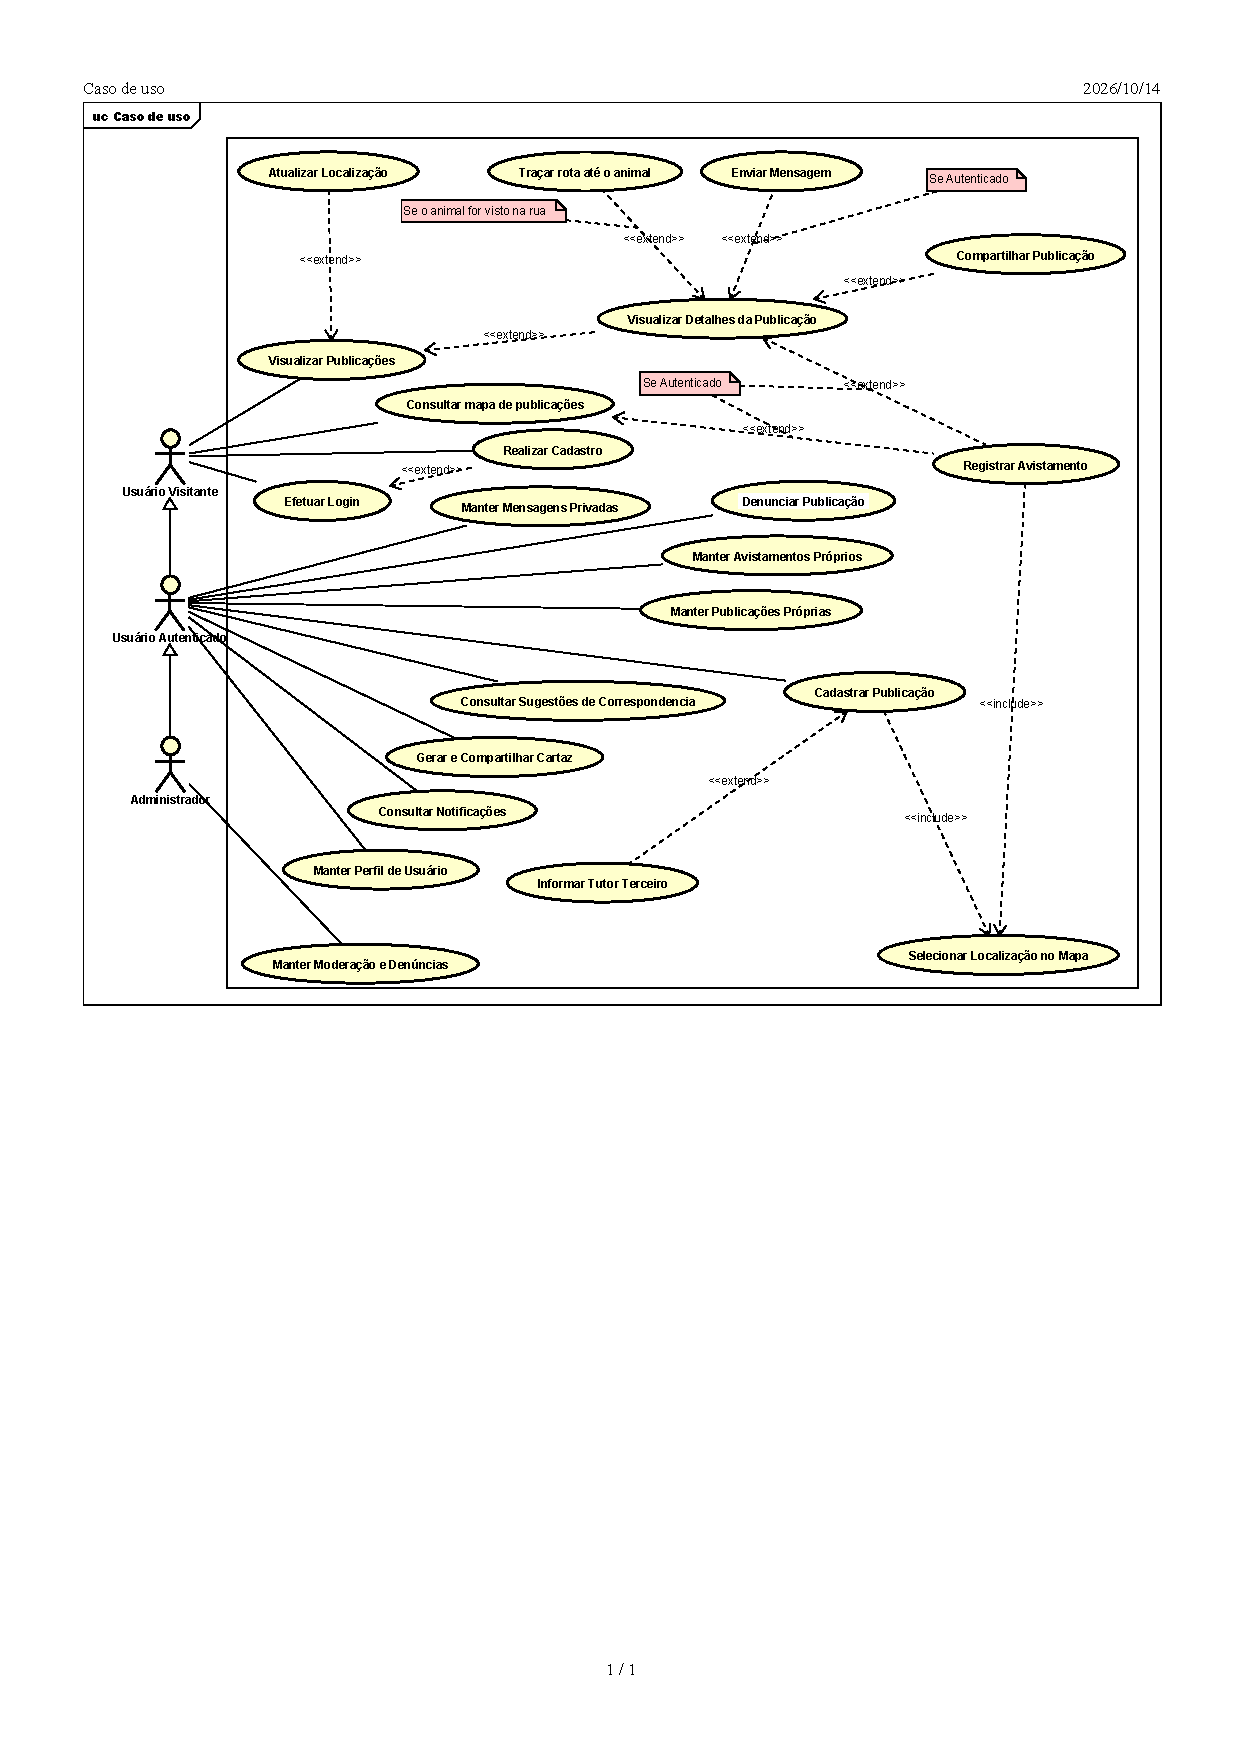
\includegraphics[
        trim=12mm 75mm 12mm 17mm,
        clip,
        width=\textwidth
    ]{imagens/02_modelagem/figura06_diagrama_casos_de_uso_reduzido.pdf}
    \vspace{-4.4cm}
    \fonte{Autoria própria (2026)}
\end{figure}

O diagrama apresenta três atores em uma hierarquia: o usuário autenticado especializa o usuário visitante e, por isso, herda suas funções; o administrador, por sua vez, especializa o usuário autenticado e também pode executar as ações disponíveis a esse perfil. O visitante pode consultar e pesquisar publicações, visualizar o mapa e os detalhes dos anúncios, criar uma conta e entrar no sistema. Ao se autenticar, passa a poder cadastrar publicações e manter as próprias publicações e os próprios avistamentos, além de utilizar mensagens privadas, consultar notificações e sugestões de correspondência, gerar cartazes, denunciar publicações e manter seu perfil. O administrador também pode moderar conteúdo e analisar denúncias.

As relações de inclusão indicam etapas obrigatórias: tanto o cadastro de uma publicação quanto o registro de um avistamento incluem a seleção da localização no mapa. Já a informação de dados de um responsável de terceiro estende o cadastro de publicação quando essa situação se aplica. A visualização dos detalhes pode ser complementada por ações opcionais, como traçar uma rota, enviar uma mensagem, compartilhar a publicação ou registrar um avistamento. A opção de atualizar a localização também complementa a consulta das publicações. O diagrama resume as funções centrais; regras de negócio e fluxos alternativos são especificados no Quadro 2 e no Apêndice A.


\subsubsection{Diagrama de Classes de Domínio}

O diagrama de classes de domínio organiza as entidades da aplicação, seus atributos, operações e relações. A Figura~\ref{fig:diagrama_classes} apresenta uma visão resumida do modelo implementado, concentrada nas entidades diretamente relacionadas aos fluxos de publicação, avistamento, comunicação e moderação.

\begin{figure}[H]
    \centering
    \caption{Diagrama de Classes de Domínio do Sistema Proposto}
    \label{fig:diagrama_classes}
    \vspace{0.3cm}
    \includegraphics[trim=12mm 95mm 12mm 8mm, clip, width=0.99\textwidth]{imagens/02_modelagem/figura08_diagrama_classes.pdf}
    \vspace{0.8cm}
    \fonte{Autoria própria (2026)}
\end{figure}

\enlargethispage{2\baselineskip}
No modelo, \textit{Usuario} representa as contas e concentra os dados e operações de autenticação, perfil e participação na plataforma. \textit{Publicacao} representa os registros de animais, reunindo categoria, situação, descrição, localização, características e operações de criação, edição, encerramento, renovação e compartilhamento. A classe \textit{Avistamento} registra relatos associados a uma publicação, enquanto \textit{FotoPublicacao} organiza as imagens vinculadas a esse registro.

A comunicação privada é representada pelas classes \textit{Conversa} e \textit{Mensagem}. A classe \textit{Denuncia} apoia o envio e o tratamento administrativo de denúncias relacionadas às publicações. A classe \textit{Devolucao} representa o fluxo de solicitação e resposta relacionado à devolução ou à entrega do animal, conforme o estado indicado no modelo. As associações e multiplicidades apresentadas na figura indicam os vínculos entre usuários, publicações, avistamentos, imagens, conversas, mensagens, devoluções e denúncias; os métodos foram mantidos na figura para evidenciar as principais operações de cada entidade.

Com os requisitos funcionais formalizados e a modelagem de classes de domínio consolidada, o Capítulo 5 apresenta a solução proposta com o aplicativo WeFIND, detalhando a concepção da ferramenta, sua arquitetura e as decisões técnicas adotadas.
